\documentclass[11pt]{article}
\usepackage{multicol}
\usepackage{graphicx}
\usepackage{todonotes}
\usepackage{tcolorbox}

\usepackage{anysize,color,float,graphicx,url,comment,hyperref,ulem}
\usepackage{hyperref}
\hypersetup{
    colorlinks=true,
    linkcolor=blue,
    filecolor=magenta,      
    urlcolor=red,
}
\usepackage{amsmath, amsfonts, amssymb}
\usepackage{enumitem}
\usepackage{HW}
\includecomment{comment}
\excludecomment{studentSpace}
\includecomment{studentSpace}

\includecomment{answer}
\excludecomment{answer}
\includecomment{comment}
\newcommand{\blank}{
\underline{\hspace{1.5cm}\hspace{1.5cm}}
}
\newcommand{\norm}[1]{\left\lVert#1\right\rVert}

\begin{document}
\titleline{\semester}
\exhead{Problem Set: Due: 10:00 PM,  18-Feb}
\begin{itemize}
\item Please write (only if true) the honor code. If you used any
  source (person or thing) explicitly state it. 

\item Important: This is an INDIVIDUAL assignment.

\item Always provide a brief explanation. (The length of the
  explanation required has been forecasted with the amount of space
  provided.)
  
\item Submit following files in folder name lab03\_roll\_XX :
	\begin{enumerate}
      \item readme.txt (case sensitive name). This \emph{text} file
        contains identifying information, honor code, links to
        references used 
      \item ReflectionEssay.pdf is optional but a brief one would be nice.
      \item lab03\_roll\_XX.pdf (includes all solutions). 
      \item All relevant tex source (and images only if necessary). No
        other junk files, please.
     \end{enumerate}
\end{itemize} 

\hrulefill
\begin{enumerate}

\begin{tcolorbox}
\item  State whether or not the following points are the same and explain why.
\begin{multicols}{2}
\begin{enumerate}[]
\item
$A[2, -1, 3]$, $B[4,-2,6]$
\item
$A[\sqrt{2}/2, -1,0]$, $B[1,-\sqrt{2},0]$
\end{enumerate}
\end{multicols}
\begin{studentSpace}
\textbf{Answer:}
\begin{enumerate}[]
\item As points lie in homogeneous coordinate system. \newline
$A = [2/3, -1/3, 1]$, $ B = [4/6,-2/6,1]=[2/3, -1/3, 1]$\newline
Therefore the two points are same.
\item Points lie in homogeneous coordinate system. \newline
$A = [\sqrt{2}/2, -1,0] = [x1,y1,w1]$, $B = [1,-\sqrt{2},0] = [x2,y2,w2]$\newline
As $w1$ and $w2$ are 0, the points $A$ and $B$ are ideal points. \newline
$(x1 , y1)$ represent the direction for the point $A$ at infinity. \newline
$(x2 , y2)$ represent the direction for the point $B$ at infinity. \newline
Direction of point $A$ unit normalised = $[1/3,-\sqrt{2}/3]$ \newline
Direction of point $B$ unit normalised = $[1/3,-\sqrt{2}/3]$ \newline
As the unit normalised direction for both points are equal, therefore they represent the same point. 
\end{enumerate}
\end{studentSpace}

\end{tcolorbox} \begin{tcolorbox}
\item In projective three-space, what are the standard homogeneous
  coordinates of (a) the origin and (b) ideal points determined by the
  intersections of the extensions of the coordinate axes and the ideal
  plane?
\begin{studentSpace}
\newline \newline
\textbf{Answer:}
\begin{enumerate}[]
\item Origin = $[0,0,0,1]$
\item Intersection of ideal plane $p$ with x-axes is $[x,0,0,0]$ \newline 
Intersection of ideal plane $p$ with y-axes is $[0,y,0,0]$ \newline
Intersection of ideal plane $p$ with z-axes is $[0,0,z,0]$ \newline  
\end{enumerate}
\end{studentSpace}
\end{tcolorbox}

\begin{tcolorbox}
\item Write standard homogeneous coordinates for the points specified
  in uppercase characters. (Use left and right to distinguish.)

\begin{minipage}{0.45\textwidth}
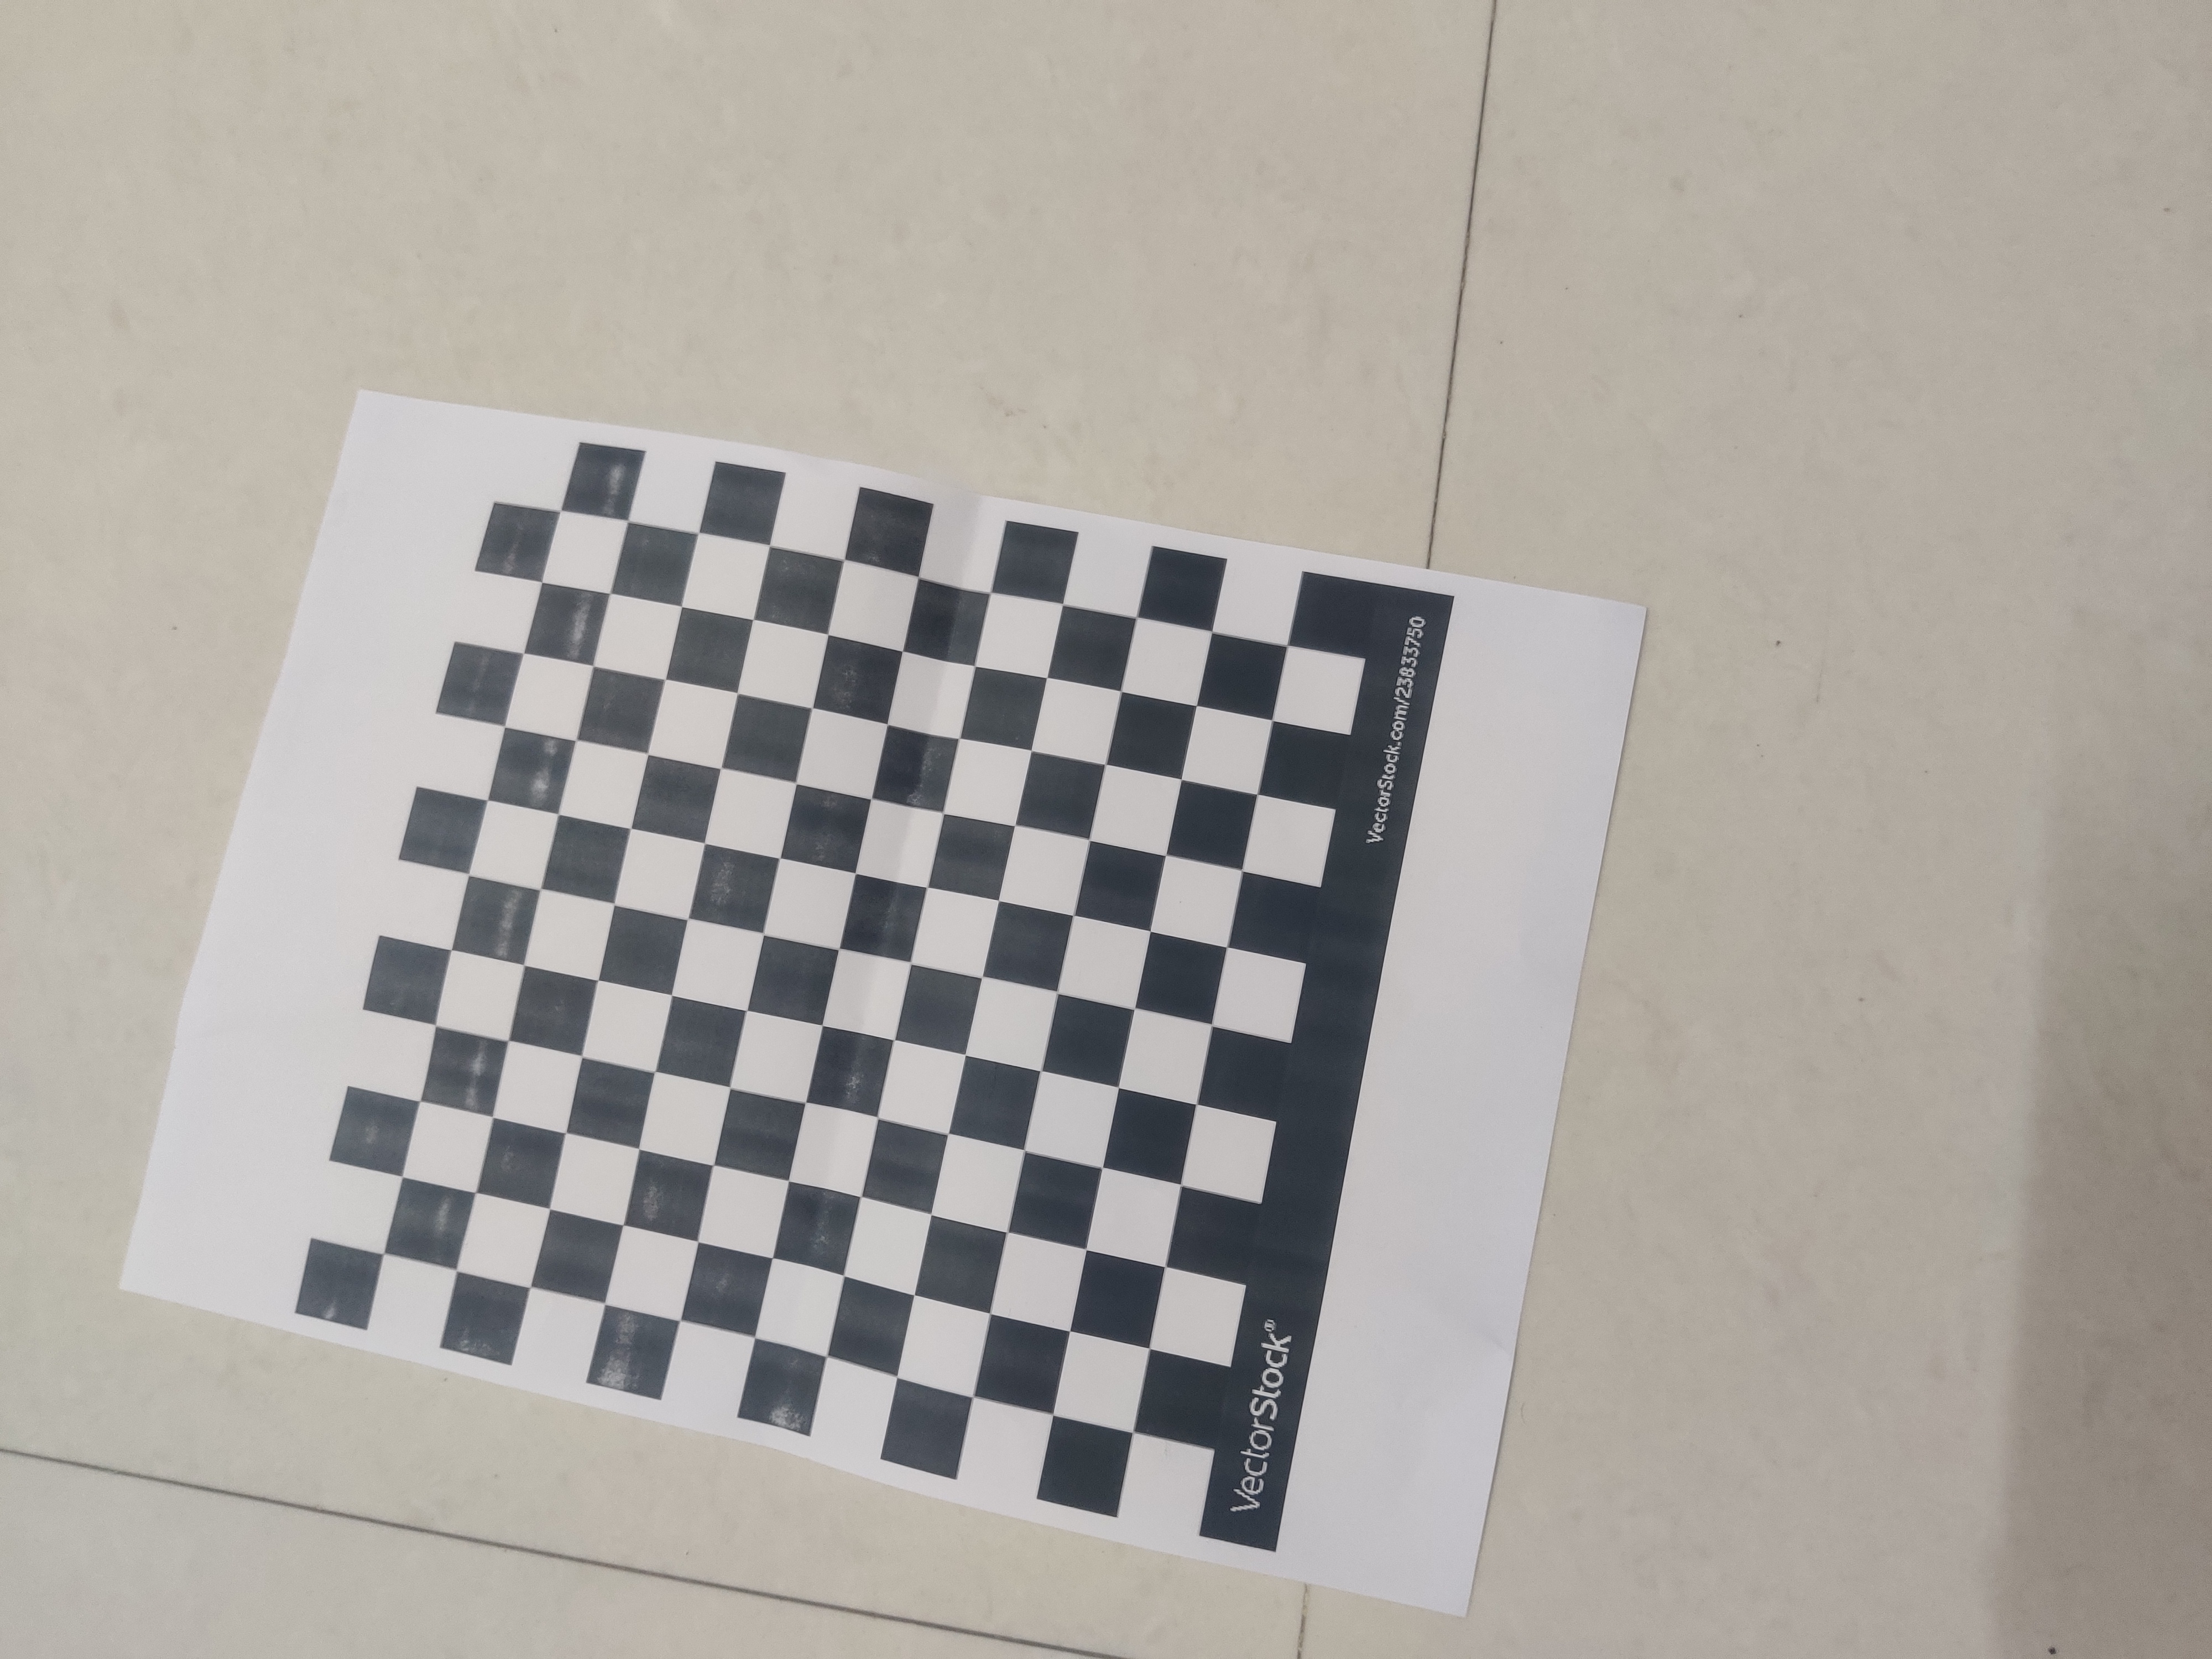
\includegraphics[width=\textwidth, height=.5\textheight,keepaspectratio]{images/image2.png}
\end{minipage} \hfill
\begin{minipage}{0.45\textwidth}
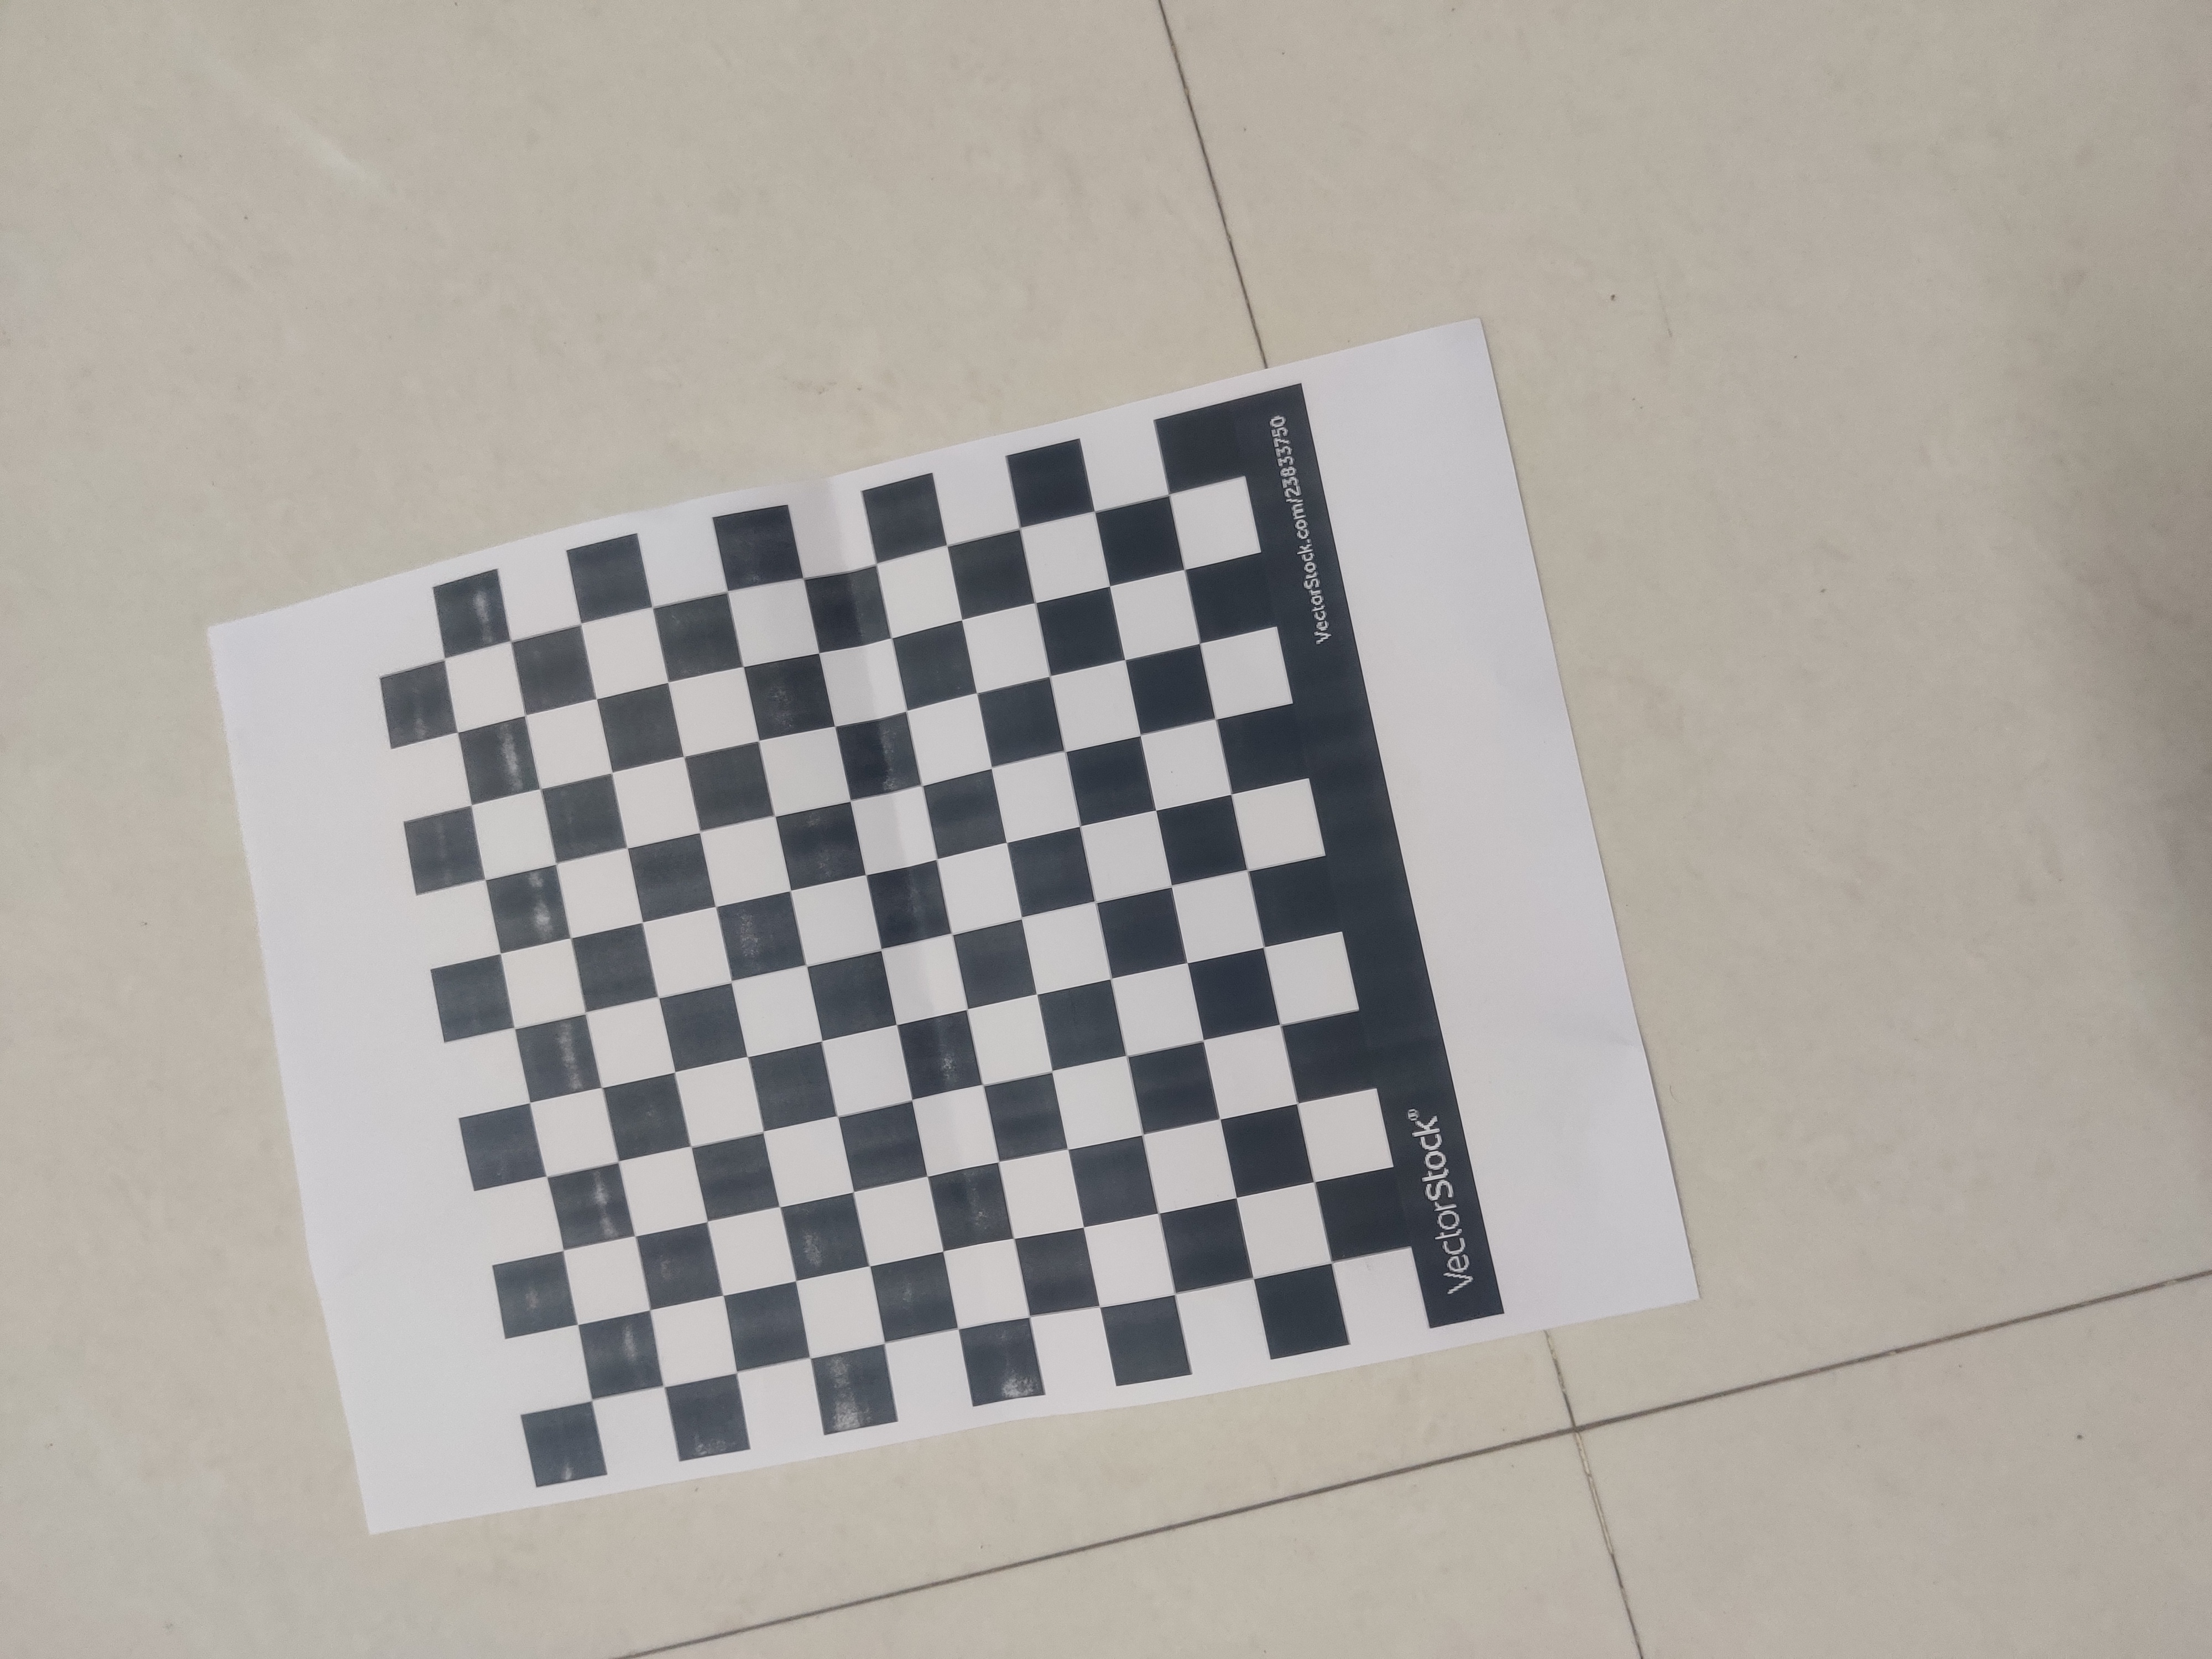
\includegraphics[width=\textwidth, height=.5\textheight,keepaspectratio]{images/image1}
\end{minipage}
\begin{studentSpace}
\newline
\textbf{Answer:} \newline
Assuming the points are in $P^2$ space. \newline
The points in homogeneous coordinate system are : \newline
$A=[0,0,1] \quad B=[2,0,1] \newline C=[3,1,1] \quad L=[1.5,-0.5,1] \newline K=[1,-4,1] \quad I=[-1,1,1] \newline J=[-4,-2,1] \quad H=[-4,3,1] \newline G=[-3,4,1] \quad E=[-1,4.5,1]$
\end{studentSpace}



\end{tcolorbox} \begin{tcolorbox}
\item Which of the following points lie on the line $3p_1 -2p_2+5p_3 =
  0$?  Why?
\begin{multicols}{2}
\begin{enumerate}[]
\item
$A[1,1,2]$
\item
$B[4,1,-2]$
\end{enumerate}
\end{multicols}
\begin{studentSpace}
  \textbf{Answer:}
  \begin{enumerate}[]
  \item Put $p_1=1, p_2=1, p_3=2$ in equation of the line  $3p_1 -2p_2+5p_3$  \newline
  $LHS = 3*1 - 2*1 + 5*2 = 11$ \newline
  $RHS = 0$ \newline
  $LHS \neq RHS $ \newline
  Therefore, the point does not lie on the line.

  \item Put $p_1=4, p_2=1, p_3=-2$ in equation of the line  $3p_1 -2p_2+5p_3$  \newline
  $LHS = 3*4 - 2*1 + 5*(-2) = 0$ \newline
  $RHS = 0$ \newline
  $LHS = RHS $ \newline
  Therefore, the point lies on the line.
  \end{enumerate}
\end{studentSpace}

\end{tcolorbox} \begin{tcolorbox}
\item Write the coordinates of the lines that are the extensions to the
  projective plane of the following Euclidean lines.
\begin{multicols}{2}
\begin{enumerate}[]
\item
$3x + 2y = 6$
\item
$4x + 5y + 7 = 0$
\end{enumerate}
\end{multicols}
\begin{studentSpace}

  \textbf{Answer:}
  \begin{enumerate}[]
  \item $ \begin{bmatrix} 3 & 2 & -6 \end{bmatrix} \begin{bmatrix} x \\ y \\ 1 \end{bmatrix} = 0 $ \newline
  Therefore, coordinates of the line that is extension to the projective plane are $[3,2,-6]$.

  \item $ \begin{bmatrix} 4 & 5 & 7 \end{bmatrix} \begin{bmatrix} x \\ y \\ 1 \end{bmatrix} = 0 $ \newline
  Therefore, coordinates of the line that is extension to the projective plane are $[4,5,7]$.

  \end{enumerate}


\end{studentSpace}

\end{tcolorbox} \begin{tcolorbox}
\item Sketch each line in the projective plane whose equation is given.
\begin{multicols}{2}
\begin{enumerate}[]
\item
$2p_1 + 3p_2 + 5p_3 = 0$
\item
$3p_1 - 2p_2 - p_3 = 0$
\end{enumerate}
\end{multicols}
\begin{studentSpace}
  \textbf{Answer:}
  \begin{enumerate}[]

    \item Put $p_3=1$ in the equation. After that equation becomes \newline
    $2p_1 + 3p_2 = -5$ \newline
    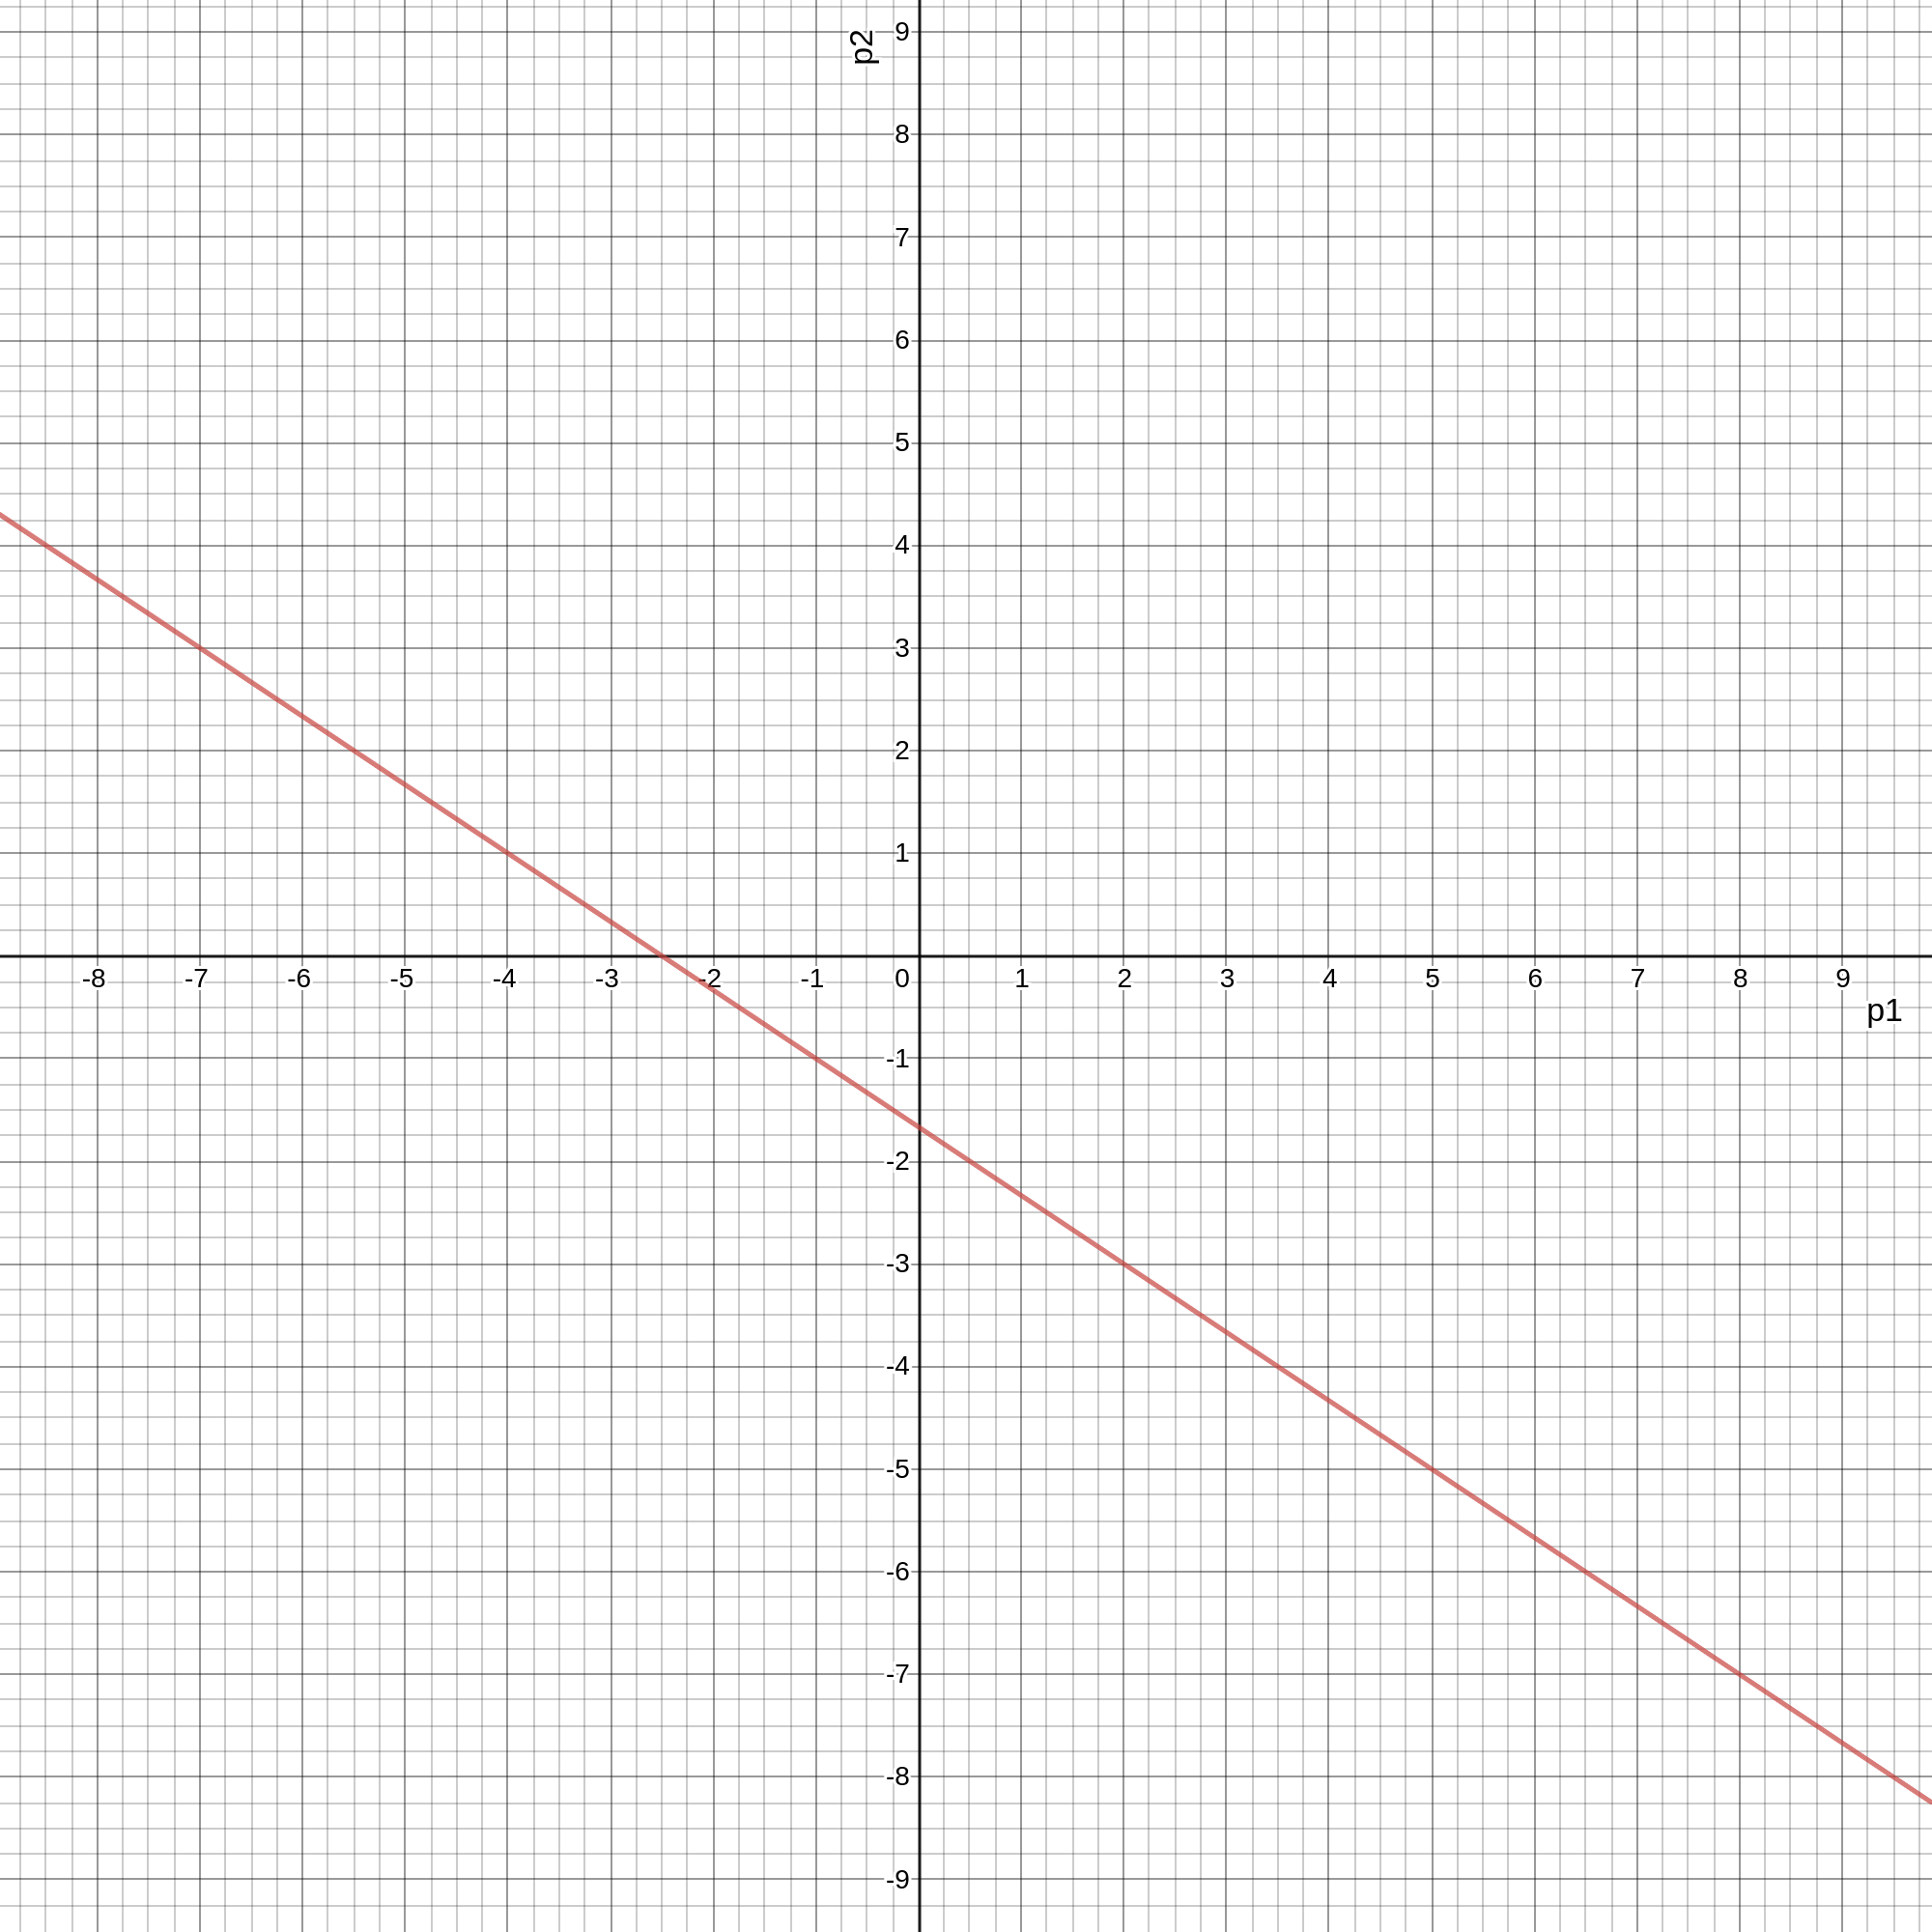
\includegraphics[width=.5\textwidth, height=.5\textheight,keepaspectratio]{./images/6a.png}

    \item Put $p_3=1$ in the equation. After that equation becomes \newline
    $3p_1 - 2p_2 = 1$ \newline
    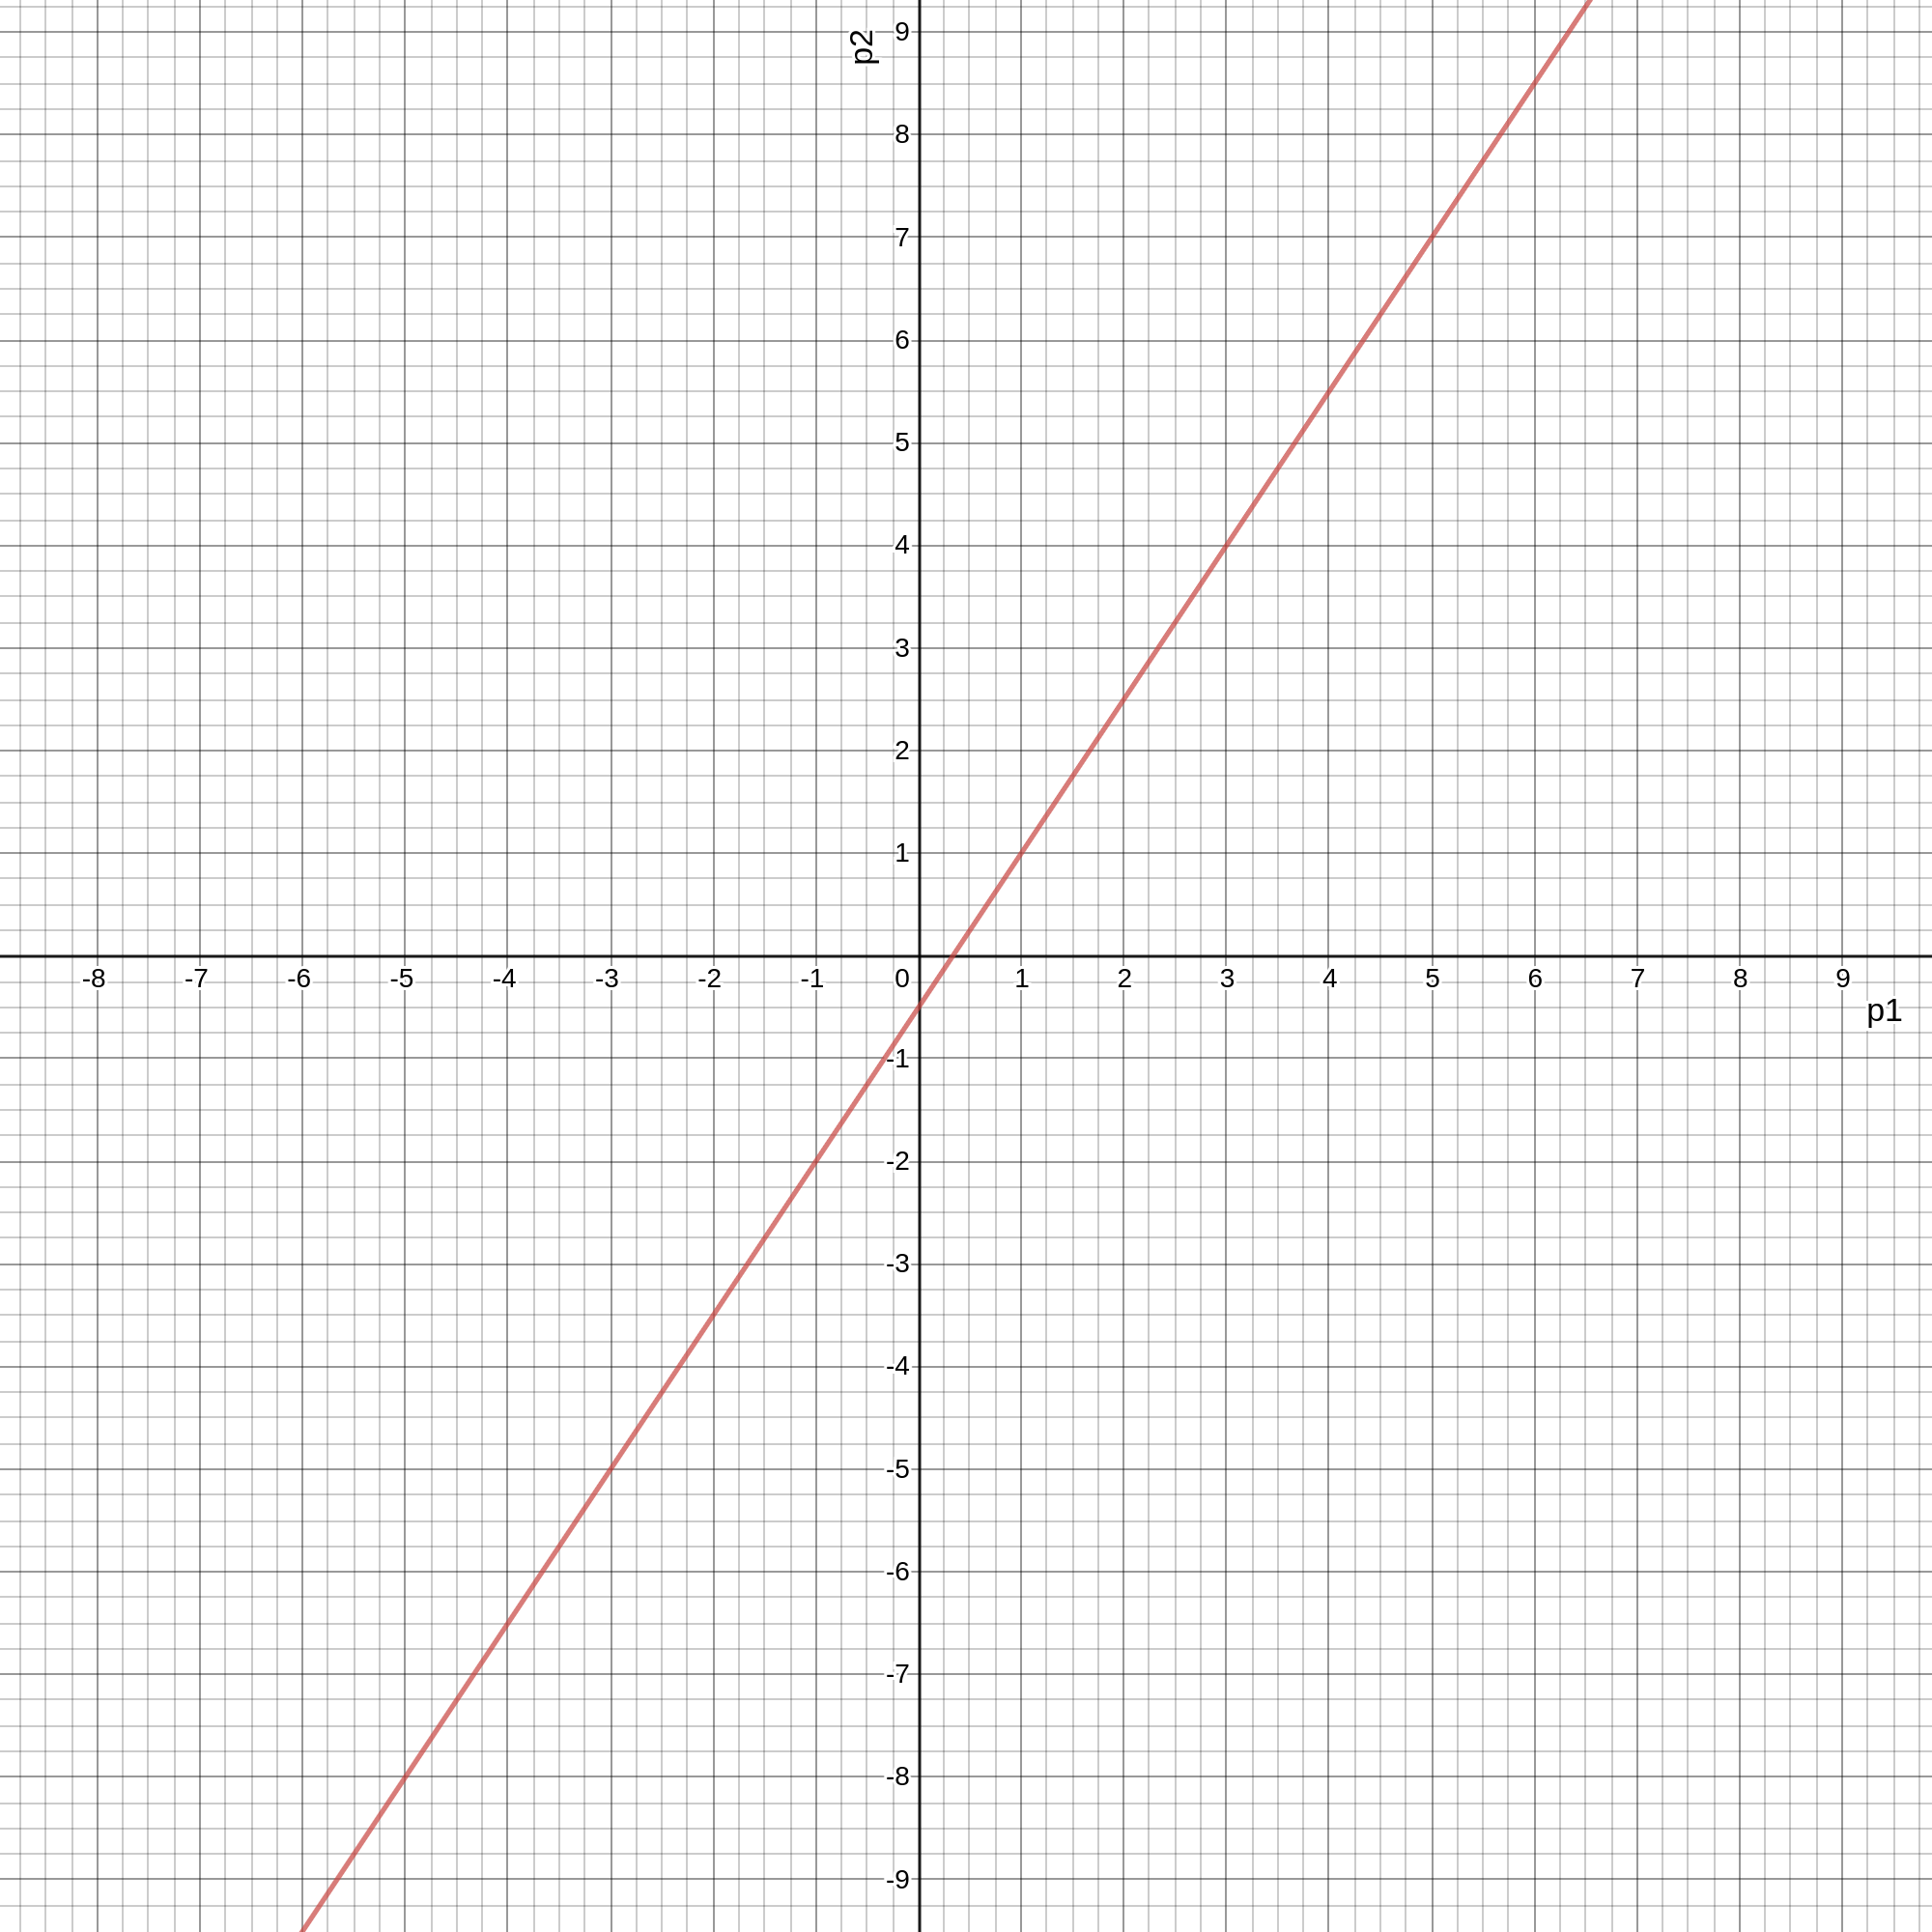
\includegraphics[height=.5\textheight, width=.5\textwidth, keepaspectratio]{./images/6b.png}
  \end{enumerate}
\end{studentSpace}
\end{tcolorbox} \begin{tcolorbox}
\item  In each of the following cases, sketch the line determined by the two given points; then find the equation of the line.
\begin{multicols}{2}
\begin{enumerate}[]
\item
$A[3, 1, 2]$, $B[1,2,-1]$
\item
$A[2,1,3]$, $B[1,2,0]$
\end{enumerate}
\end{multicols}
\begin{studentSpace}
  \textbf{Answer:}
  \begin{enumerate}[]

    \item Let the line be represented as $L = [l_1,l_2,1]$.\newline
    The equations are $3l_1 + l_2 + 2 = 0, l_1 + 2l_2 - 1 =0 $. \newline
    After solving the above equations, $ L = [-1,1,1] $. \newline
    Any point $p$ on line can be represented in homogeneous coordinate as $p=[p_1,p_2,1]$
    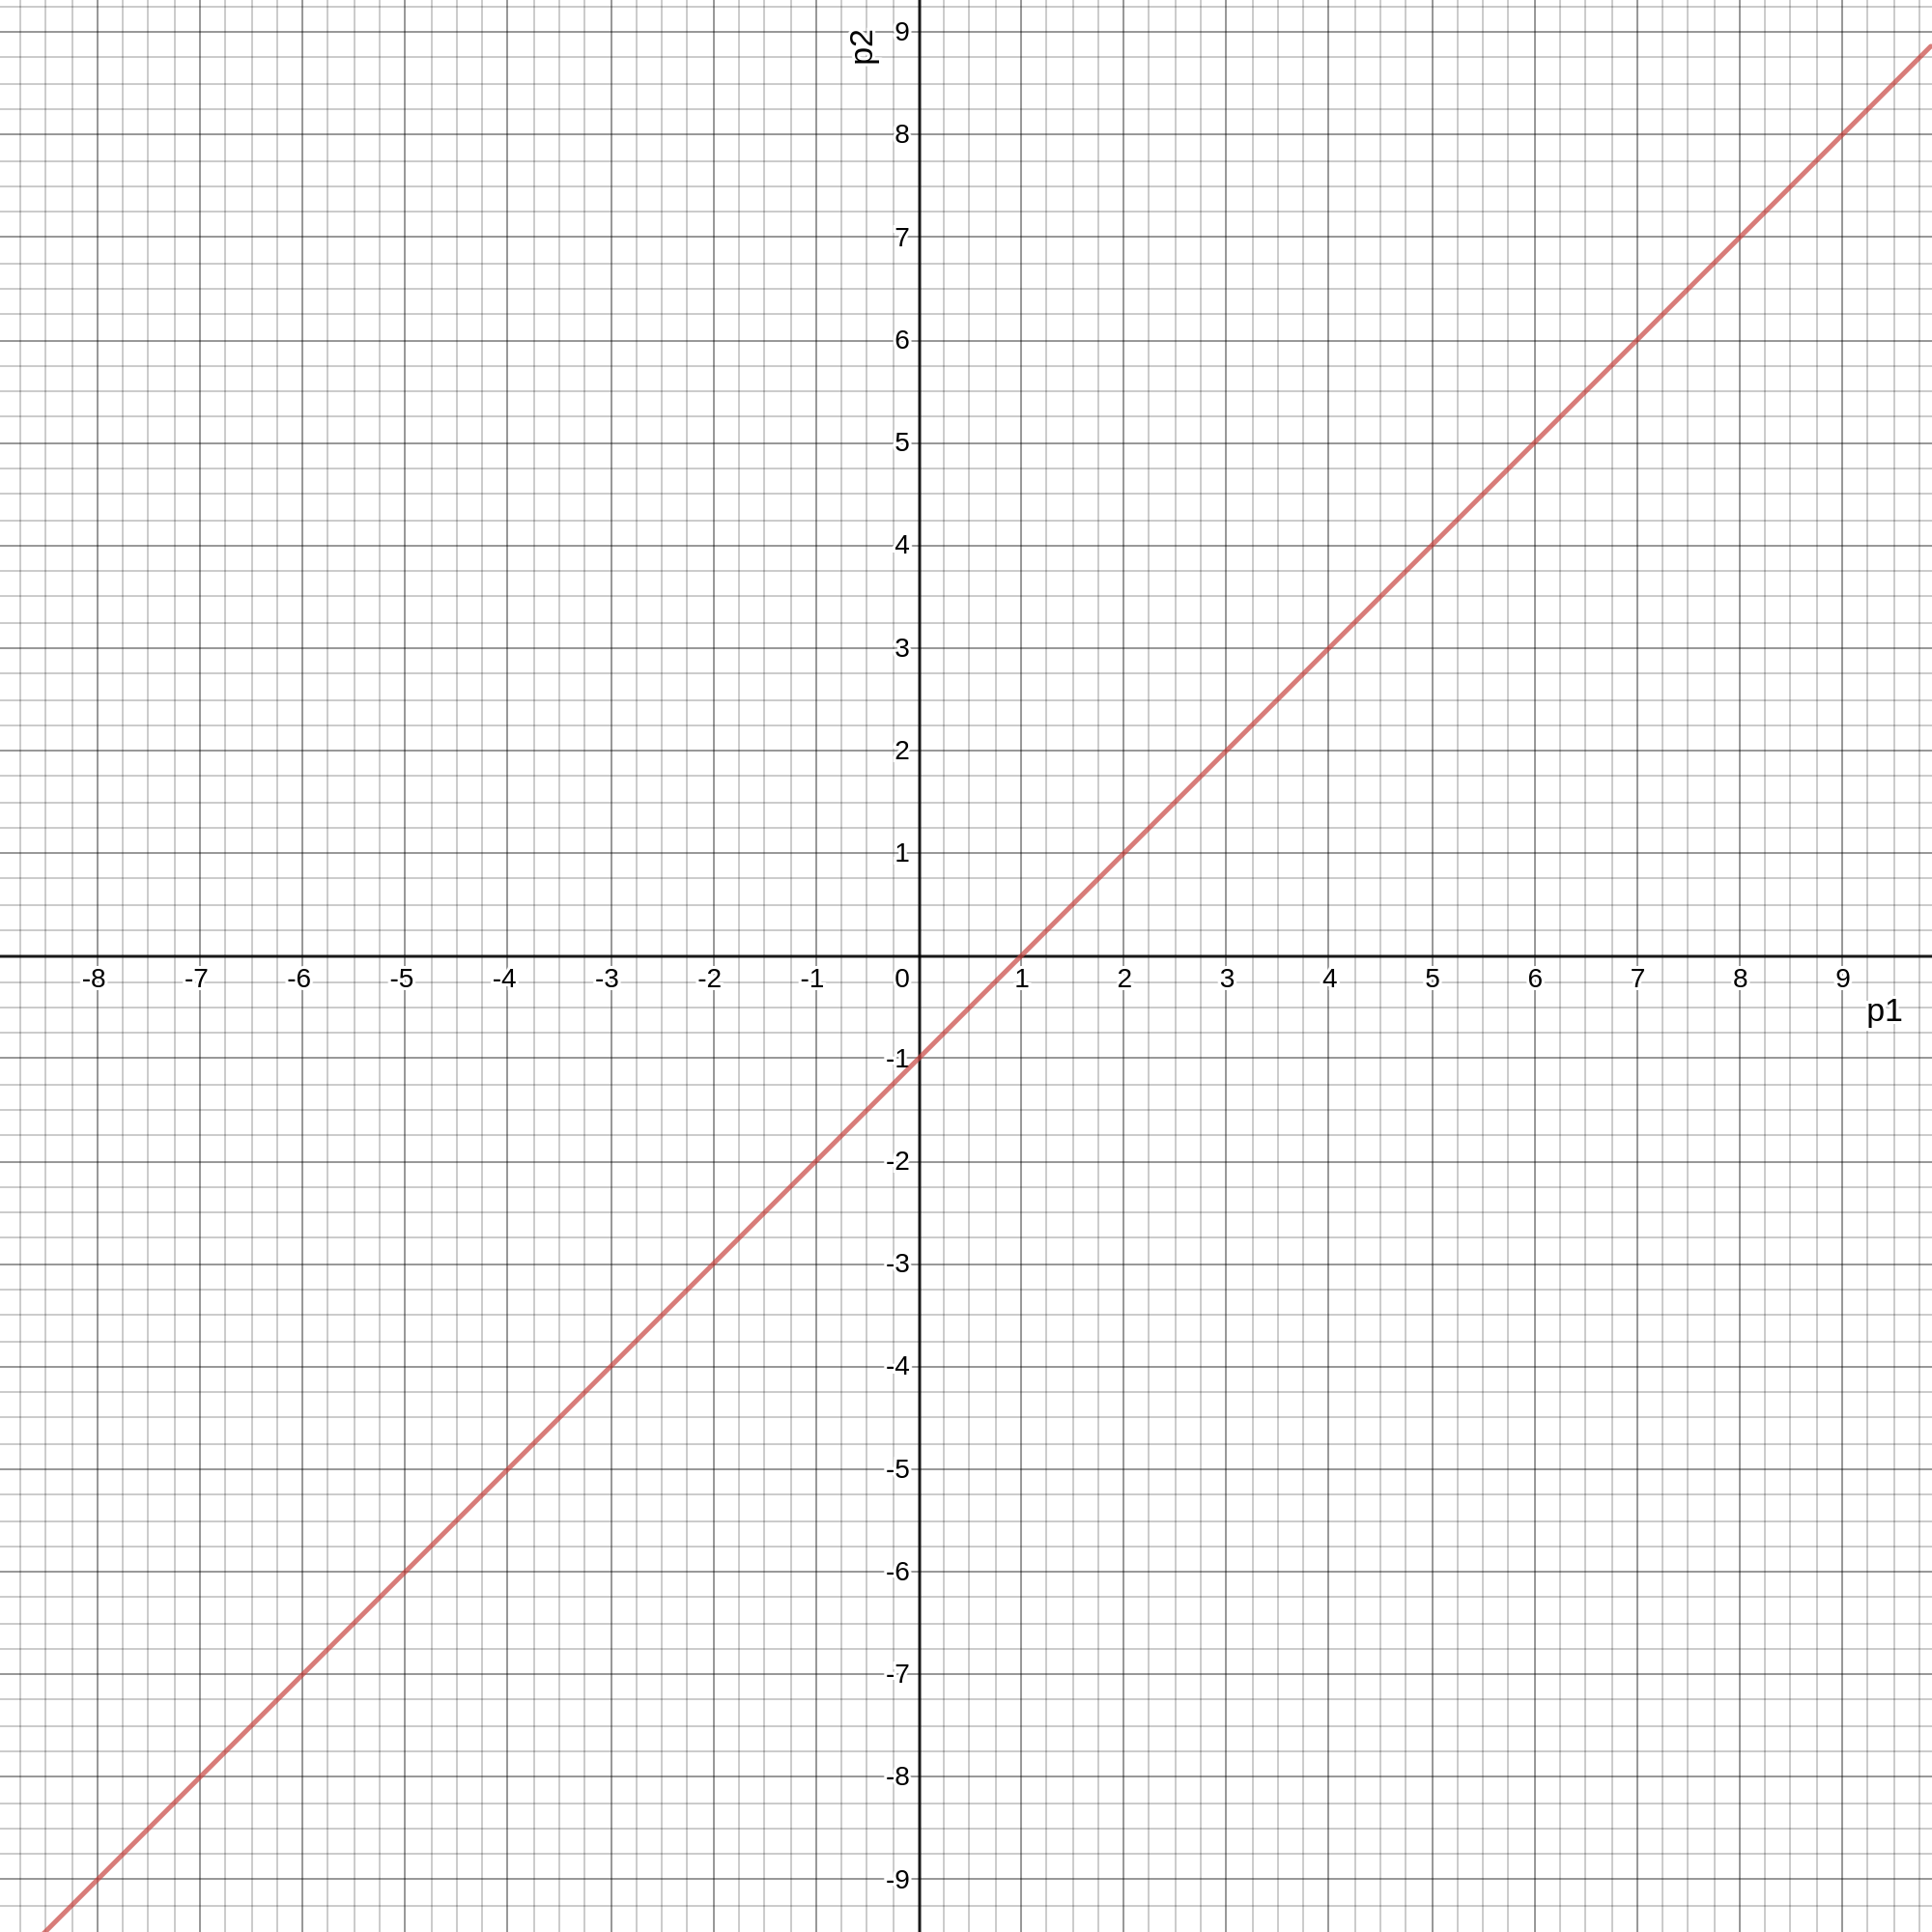
\includegraphics[width=.5\textwidth, height=.5\textheight,keepaspectratio]{./images/7a.png}

    \item Let the line be represented as $L = [l_1,l_2,1]$.\newline
    The equations are $2l_1 + l_2 + 3 = 0, l_1 + 2l_2 =0 $. \newline
    After solving the above equations, $ L = [-2,1,1] $. \newline
    Any point $p$ on line can be represented in homogeneous coordinate as $p=[p_1,p_2,1]$
    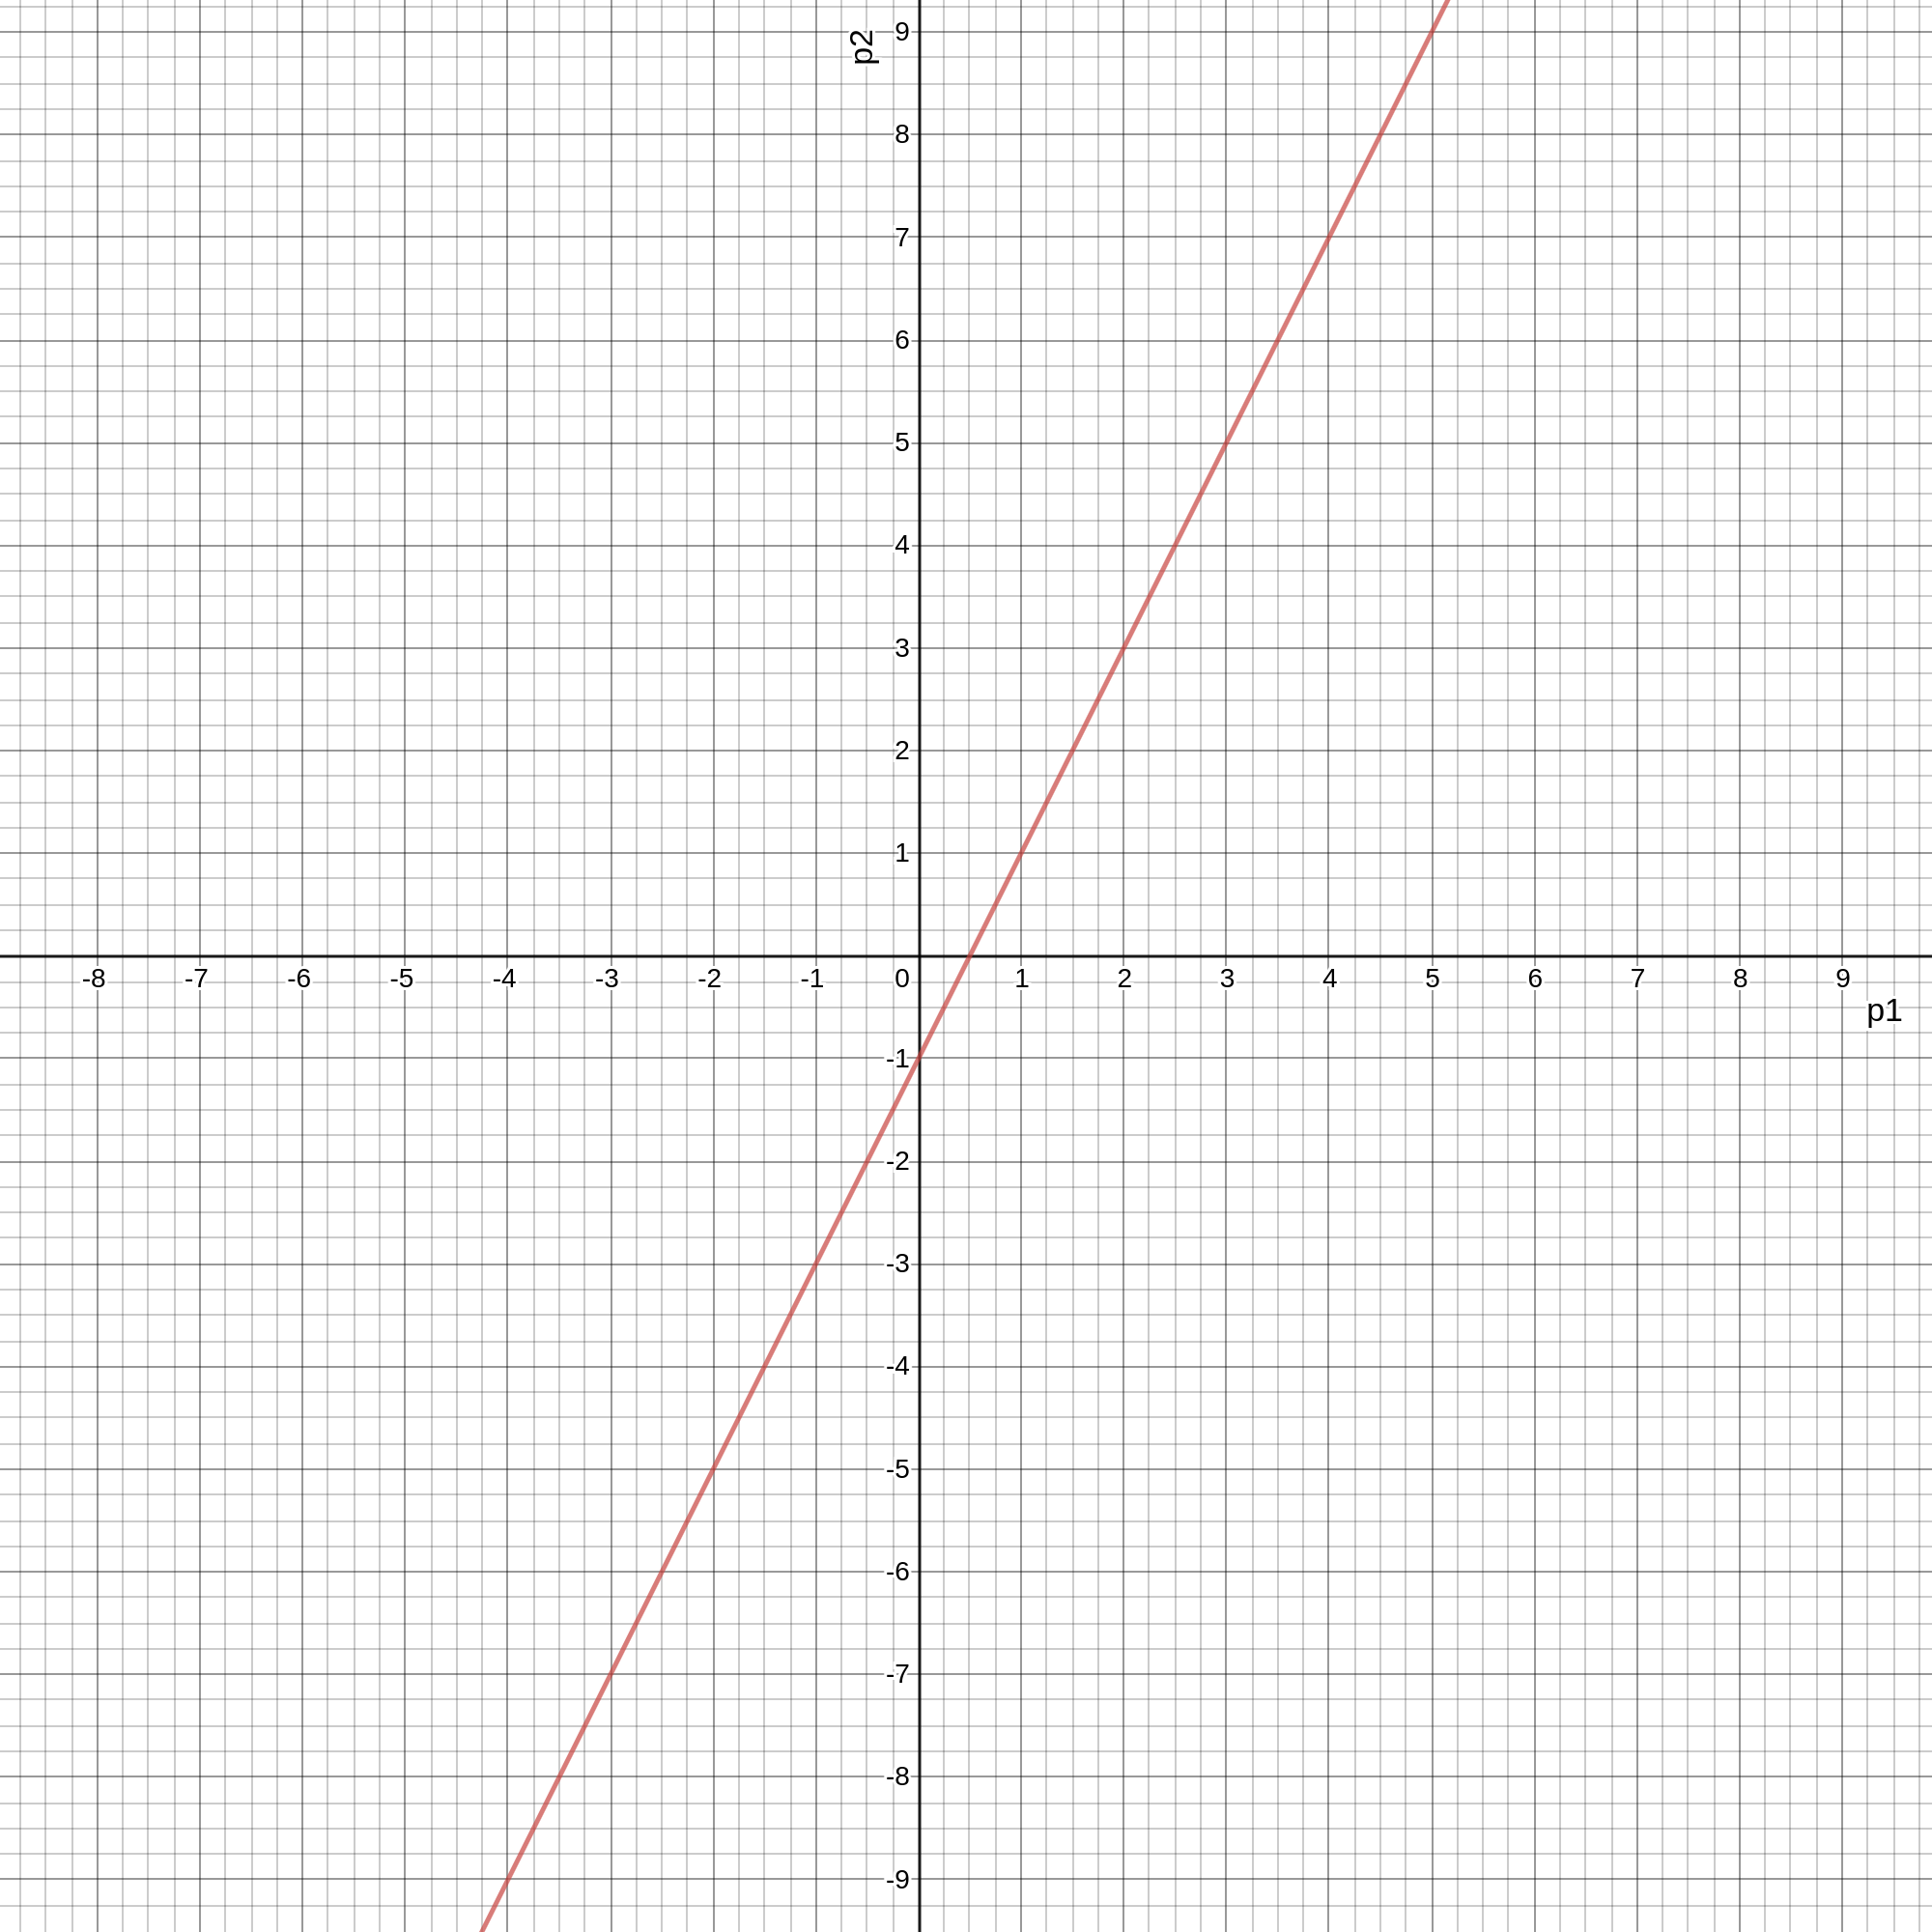
\includegraphics[height=.5\textheight, width=.5\textwidth, keepaspectratio]{./images/7b.png}
    

  \end{enumerate}
\end{studentSpace}


\end{tcolorbox} \begin{tcolorbox}
\item  Find the standard homogeneous coordinates of the point of
  intersection for each pair of lines. 
\begin{multicols}{2}
\begin{enumerate}[]
\item
$p_1 + p_2 - 2p_3 = 0, 3p_1 + p_2 + 4p_3 = 0$
\item
$p_1 + p_2 = 0, 4p_1 - 2p_2 + p_3 = 0$
\end{enumerate}
\end{multicols}
\begin{studentSpace}

  \textbf{Answer:}
  \begin{enumerate}[]

    \item For intersection of points in homogeneous coordinate system, put $p_3=1$ in the both equations and solve for $p_1$ and $p_2$. \newline
    $ p_1 + p_2 - 2*1 = 0 $ \newline
    $ 3p_1 + p_2 + 4*1 = 0 $  \newline
    After solving the above two equations, $p_1 = -3$ and $p_2 = 5$. \newline
    Therefore, the intersection of lines in homogeneous coordinates is $[-3,5,1]$ . 

    \item For intersection of points in homogeneous coordinate system, put $p_3=1$ in the both equations and solve for $p_1$ and $p_2$. \newline
    $ p_1 + p_2 = 0 $ \newline
    $ 4p_1 - 2p_2 + 1*1 = 0 $  \newline
    After solving the above two equations, $p_1 = -3$ and $p_2 = 5$. \newline
    Therefore, the intersection of lines in homogeneous coordinates is $[-1/6,1/6,1]$.

  \end{enumerate}
\end{studentSpace}


\end{tcolorbox} \begin{tcolorbox}
\item  Determine which of the following sets of three points are collinear. 
\begin{multicols}{2}
\begin{enumerate}[]
\item
$A[1,2,1]$, $B[0,1,3]$, $[2,1,1]$
\item
$A[1,2,3]$, $B[2,4,3]$, $[1,2,-2]$
\end{enumerate}
\end{multicols}
\begin{studentSpace}
  \textbf{Answer:}
  \begin{enumerate}[]

    \item $ AB = [-1,-1,2] , BC = [2,0,-2]. $ \newline
    As $ AB \neq k*BC , k $ being a real number. \newline
    Therefore, the points are not collinear.

    \item $ AB = [1,2,0] , BC = [-1,-2,-5]. $ \newline
    As $ AB \neq k*BC , k $ being a real number. \newline
    Therefore, the points are not collinear.
  \end{enumerate}

  
\end{studentSpace}

\end{tcolorbox} \begin{tcolorbox}
\item  Determine which of the following sets of three lines meet in a
  point. 
\begin{multicols}{2}
\begin{enumerate}[]
\item
$l[1,0,1], m[1,1,0], n[0,1,-1]$
\item
$l[1,0,-1], m[1,-2,1], n[3,-2,-1]$
\end{enumerate}
\end{multicols}
\begin{studentSpace}
  \textbf{Answer:}
  \begin{enumerate}[]

    \item Let $L = \begin{bmatrix} l  \\ m \\ n \end{bmatrix} $ \newline
      $L = \begin{bmatrix} 1 & 0 & 1 \\ 1 & 1 & 0 \\ 0 & 1 & -1 \end{bmatrix}$ \newline
      Let $x$ be the point which is on all three lines. Then $Lx=0$ \newline
      If $|L|=0$, then all three lines intersect in one point. \newline
      $ L = 1*(1*(-1) - 0*1) - 0*(1*(-1)-0*0) + 1*(1*1-0*1) = 0 $ \newline
    Therefore, the lines intersect in one point.

    \item Let $L = \begin{bmatrix} l  \\ m \\ n \end{bmatrix} $ \newline
      $L = \begin{bmatrix} 1 & 0 & -1 \\ 1 & -2 & 1 \\ 3 & -2 & -1 \end{bmatrix}$ \newline
      Let $x$ be the point which is on all three lines. Then $Lx=0$ \newline
      If $|L|=0$, then all three lines intersect in one point. \newline
      $ L = 1*((-2)*(-1)-(-2)*1) - 0 + (-1)*(1*(-2)-(-2)*(3)) = 0 $ \newline
    Therefore, the lines intersect in one point.

  \end{enumerate}
\end{studentSpace}
\end{tcolorbox}

\end{enumerate}
\end{document}

